\documentclass[11pt,addpoints]{exam}

\usepackage{tikz}
\usepackage{tkz-tab}
\usepackage[margin=2cm]{geometry}
\usepackage{amsmath}

\begin{document}

\begin{center}
    \Huge{Interrogation sur les dérivées et leurs applications}
\end{center}

\vfill

\begin{questions}

\question[3] Recopier et compléter les phrases suivantes
\begin{parts}
    \part << Soit $f$ une fonction définie et dérivable sur un intervalle ouvert $I$. Si $f'$, la fonction dérivée de $f$, est positive sur $I$ alors $f$ est .............. sur $I$. >>
    \part << Soit $g$ une fonction définie et dérivable sur un intervalle ouvert $I$. Si $g$ est décroissante sur $I$ alors $g'$, la fonction dérivée de $g$, est .............. sur $I$. >>
    \part << Soit $h$ une fonction définie et dérivable sur un intervalle ouvert $I$. Si $h$ admet un extremum en $x_O$ alors $f'(x_0)$ ........... >>
\end{parts}

\question[3] Dans chacun des cas ci-dessous, on donne la courbe représentative d'une fonction définie sur $[-3;3]$. Par lecture graphique, dresser les tableaux de variations de ces fonctions en y incluant le signe de leur fonction dérivée.

\begin{center}
    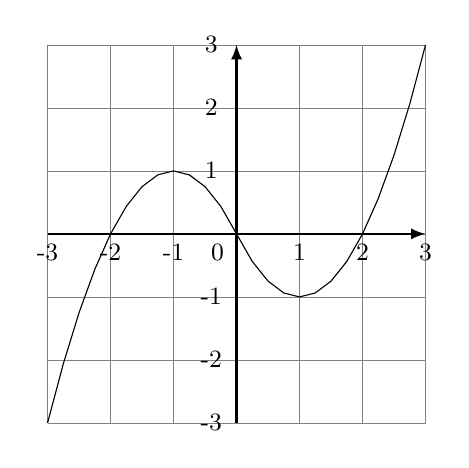
\begin{tikzpicture}[scale=0.8,domain=-3:3]
        \draw[line width=0.03mm, gray] (-3,-3) grid (3,3);
        \draw[thick, -latex] (-3,0) -- (3,0);
        \draw[thick, -latex] (0,-3) -- (0,3);
        \node at (-0.3,-0.3) {\small 0};
        \foreach \x in {1,2,3} 
        {
            \node at (\x,-0.3) {\small \x};
            \node at (-\x,-0.3) {\small -\x};
            \node at (-0.4,\x) {\small \x};
            \node at (-0.4,-\x) {\small -\x};
        }
        \draw plot(\x,{\x^2-2*\x});
    \end{tikzpicture}
    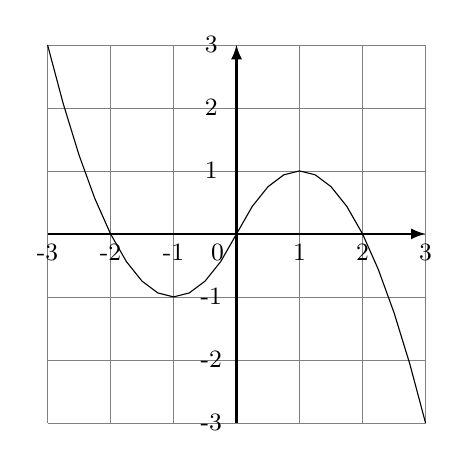
\begin{tikzpicture}[scale=0.8,domain=-3:3]
        \draw[line width=0.03mm, gray] (-3,-3) grid (3,3);
        \draw[thick, -latex] (-3,0) -- (3,0);
        \draw[thick, -latex] (0,-3) -- (0,3);
        \node at (-0.3,-0.3) {\small 0};
        \foreach \x in {1,2,3} 
        {
            \node at (\x,-0.3) {\small \x};
            \node at (-\x,-0.3) {\small -\x};
            \node at (-0.4,\x) {\small \x};
            \node at (-0.4,-\x) {\small -\x};
        }
        \draw plot(\x,{-\x^2+2*\x});
    \end{tikzpicture}
    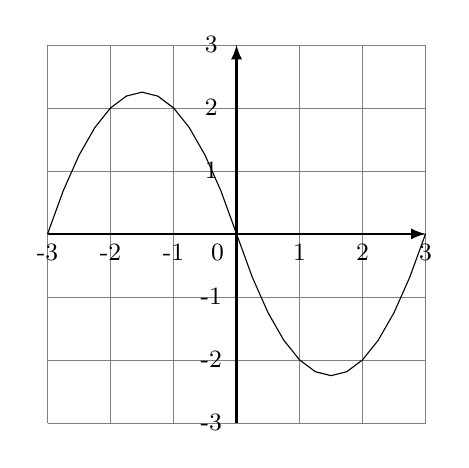
\begin{tikzpicture}[scale=0.8,domain=-3:3]
        \draw[line width=0.03mm, gray] (-3,-3) grid (3,3);
        \draw[thick, -latex] (-3,0) -- (3,0);
        \draw[thick, -latex] (0,-3) -- (0,3);
        \node at (-0.3,-0.3) {\small 0};
        \foreach \x in {1,2,3} 
        {
            \node at (\x,-0.3) {\small \x};
            \node at (-\x,-0.3) {\small -\x};
            \node at (-0.4,\x) {\small \x};
            \node at (-0.4,-\x) {\small -\x};
        }
        \draw plot(\x,{\x^2-3*\x});
    \end{tikzpicture}
\end{center}

\question[6] Déterminer le(s) extremum(s) locaux des fonctions, préciser leur nature (maximum ou minimum)
\begin{parts}
    \part $f$ définie sur $]-\infty;+\infty[$ par $f(x) = 3x^2+2x+7$
    \part $g$ définie sur $[0;+\infty[$ par $g(x) = \sqrt{x} - x$
    \part $h$ définie sur $]-\infty;+\infty[$ par $h(x) = (x-2)(-3x^2+5)$
\end{parts}

\question[5]

Soit la fonction $f$ définie telle que $f(x) = 1 + \dfrac{4}{(x-1)} + \dfrac{3}{(x-1)^2}$.
\begin{parts}
    \part Donner l'intervalle sur lequel $f$ est définie et dérivable
    \part On donne que $\lim\limits_{x\to-\infty} f(x) = 1$ et $\lim\limits_{x\to+\infty} f(x) = 1$\\
    Dresser le tableau de variations de $f$.
    \part Combien y aura-t-il de solutions à l'équation $f(x) = 0$ ? Expliquer.
\end{parts}

\question[3] Une entreprise fabrique des boîtes de conserve de 1 $dm^3$ en fer-blanc à forme cylindrique. Quelles dimensions doivent avoir ces boites de conserve afin d'utiliser le moins de fer-blanc possible ?

\hqword{Exercice}
\begin{center}
\gradetable[h][questions]
\end{center}

\end{questions}
\end{document}